\documentclass[13pt]{article}
%Gummi|065|=)
\title{\textbf{ARREGLOS Y PARAMETROS DE LOS AMPLIFICADORES CLASE B.}}
\author{Jaime Guzman}
\usepackage{graphicx}
\begin{document}
\date{octubre 8}
\begin{figure}[htp]
\centering

\includegraphics[scale=1.00]{IMAGENES/índice.png}
\caption{}
\label{}
\end{figure}
\maketitle

\section{Caracteristicas}

Se les denomina amplificadores de clase B cuando el voltaje de polarizacion y la amplitud maxima de la señal poseen valores que hacen que la corriente de la salida circule durante el semiciclo de la señal de entrada.\\
su principal caracteristica es que puede amplificar en muy alto nivel.\\
Tambien tomando en cuenta a los amplificadores del tipo AB que son la mezcla entre los dos anteriores cuando el voltaje de polarizacion y la maxima amplitud de la señal entrante poseen valores que hacen que la corriente de la salida circule durante menos ciclo completo y mas de la mitad del ciclo de la señal de entrada, se les denomina: Amplificadores de potencia clase AB.\\\\

Algunas de las principales ventajas de estos amplificadores es que poseen un bajo consumo en reposo lo que se refiere a un consumo mas eficiente de energia y un mejor rendimiento electrico, otra de las ventajas mayores de esta configuracion de amplificadores es que la corriente que es entregada al amplificador es la que se utiliza, es decir tiene un gran rendimineto de corriente.\\
Otra de las ventajas es que cuando este esta en reposo su intensidad es casi nula puesto que no requiere casi intensidad cuando esta en reposo ademas de ser eficiente.\\\\

Las desventajas que podrian afectar a su rendimiento y eficiencia podrian ser que producen cuestiones llamadas armonicos, y es mayor cuando no tienen transistores de salida con las mismas caracteristicas tecnicas, debido a que se suelen polarizar de forma que se les introduce una pequeña polarizacion directa con esto se consigue solucionar parcialmente este problema ya que con esto se consigue desplazar las curvas y se disminuye la distorcion.\\\\

\begin{figure}[htp]
\centering
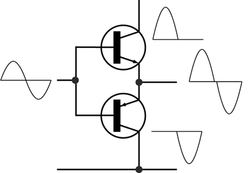
\includegraphics[scale=0.50]{IMAGENES/250px-Electronic_Amplifier_Push-pull.png}
\caption{}
\label{}
\end{figure}


Esto amplificadores son muy utilizados en cuestiones como lo podrian ser sistemas telefonicos, transistores de seguridad portatil y sistemas de aviso, estos no son muy utilizados en audio debido a que producen la mencionada anteriormente distorcion que reduce la calidad del audio.


\section{funcionamiento}

un amplificador de potencia B funciona cuando la polarizacion de dc deja al transistor casi apagado  de manera que el transistor se enciende cuando a este se le aplica una señal AC , es decir que el transistor coducira corriente solamente para una mitad del ciclo de la señal.\\\\

\begin{figure}[htp]
\centering
\includegraphics[scale=1]{IMAGENES/índice1.png}
\caption{}
\label{}
\end{figure}

Ahora para obtener una señal  del ciclo completo sera necesario utilizar dos transistores y lograr que cada uno de ellos conduzca durante medios ciclos opuestos y al tenerlos combiados que se obtenga la onda de señal completa.\\\\\\
\begin{figure}[htp]
\centering
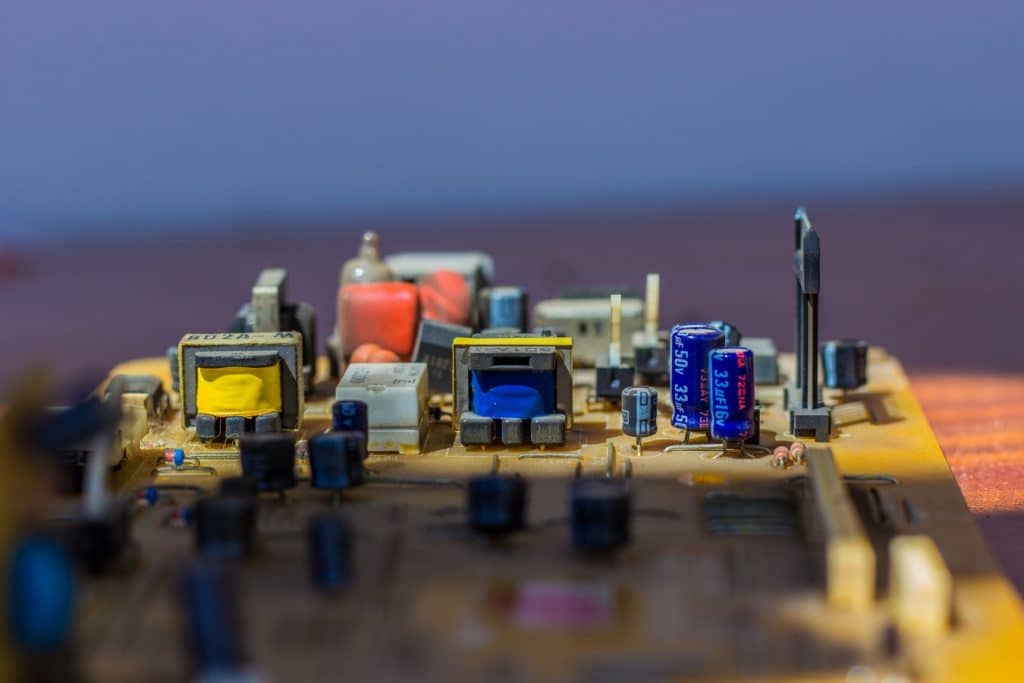
\includegraphics[scale=0.40]{IMAGENES/electronica-1024x683.jpg}
\caption{}
\label{}
\end{figure}
\section{conclusiones}
Estos tipos de amplificadores son muy caracteristicos debido a que resaltan por las caracteristicas mas importantes como serian que su estado en reposo gasta muy pocos recursos haciendo que sean muy eficientes al momento de tener que estar grandes cantidades de tiempo estando en reposo ademas de ser muy eficientes para la corriente pues esta es utilizada al maximo practicamente lo que lo hace un muy buen componente en cuanto a eficiencia supone con respecto a los amplificadores de clase A que estos tienen muy baja eficiencia.\\ siendo aproximadamente del 30 porciento de rendimiento ademas de sobrecalentarse de manera exagerada, pero los amplificadores de clase A no son remplazados por los clase B puesto que tienen una gran desventaja, estos, los amplificadores clase B tienen cierta distorsion al momento de la salida de la señal.\\ esto como se menciono anteriormente puede ser atenuada mas no eliminada puesto que por esta gran deficiencia no es el amplificador ideal para cualquier tipo de amplificacion, puesto a esto no es utilizada en componenetes de audio pues generaria la distrocion que afectaria el rendimiento de el audio, esto es el punto principal de la amplificacion de clase A que puede generar una gran fidelidad de amplificacion a cambio de eficiencia. 
 
\section{Referencias}
ecured.cu\\
cdn.usc.edu.co 

\end{document}
